\documentclass[12pt,a4paper,fleqn]{article}
\usepackage[utf8]{inputenc}
\usepackage[russian]{babel}
\usepackage{amssymb, amsmath, multicol}
\usepackage{enumitem}
\usepackage{lipsum}
\usepackage{euler}
\oddsidemargin=-15.4mm
\textwidth=190mm
\headheight=-32.4mm
\textheight=277mm
\parindent=0pt
\parskip=8pt
\pagestyle{empty}
\usepackage{graphicx}
\title{\textbf{\LARGE{Исследовательская работа по теме:\\Исследование функции дифференциальными методами}}}
\author{Известный гражданин}
\date{November 2022}
\addt\captionsrussian{\def\refname{Список литературы}}\begin{document}
\maketitle
\newpage\newpage \textbf{\LARGE{Глава I. Функция}}

\begin{center}
$y = $$sin(x)$

\end{center}
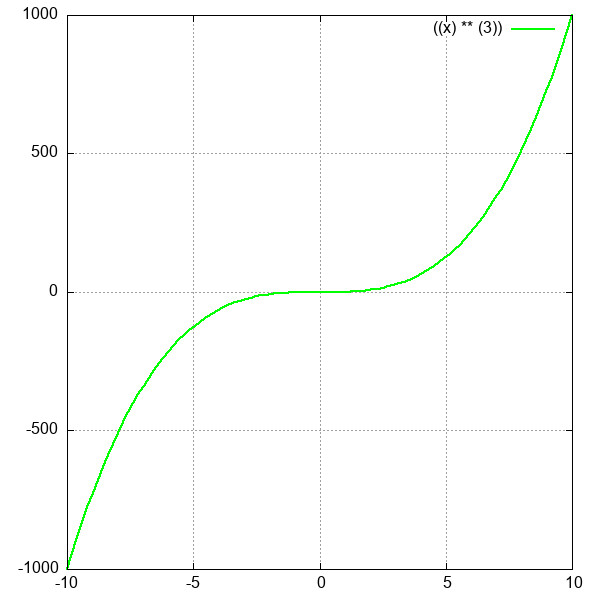
\includegraphics{GraphicDumps/plot.jpg}\newpage \textbf{\LARGE{Глава II. Визуальный анализ функции}}

Хорошо там, где производной нет\cite{link2}

\begin{center}
$y = $$sin(x)$

\end{center}
\newpage \textbf{\LARGE{Глава III. Дифференцирование}}

Ну ты же всё равно не будешь это проверять

\begin{center}
 ($x)'
  = 1$\end{center}
В ближайшее время ожидаются осадки из ваших слёз от попыток понять этот переход

\begin{center}
 ($sin(x))'
  = 1 \cdot cos(x)$\end{center}
\newpage \textbf{\LARGE{Глава IV.Упрощение выражения}}

Спешка нужна только в армии и при ловле блох. Но не как уж ни при вычислении производной\cite{link2}

\begin{center}
$1 \cdot cos(x) = cos(x)$\end{center}
\newpage \textbf{\LARGE{Глава V. Полученая производная}}

$y = $$sin(x)$

$y' = $$cos(x)$

\includegraphics{GraphicDumps/plot_1.jpg}\newpage \textbf{\LARGE{Глава VI. Разложение функции по формуле Тейлора}}

Паршивая функция всё доказательство портит\cite{link2}

\begin{center}
\end{center}
\begin{center}$sin(0) = 0$\end{center}
Обоснование этого пререхода предостовляется читателю в платном DLC

\begin{center}
 ($x)'
  = 1$\end{center}
Дифференциал от производной не далеко падает\cite{link2}

\begin{center}
 ($sin(x))'
  = 1 \cdot cos(x)$\end{center}
Используя выводы из теоремы 1000-7 получаем

\begin{center}
$1 \cdot cos(x) = cos(x)$\end{center}
Руководствуясь базовой логикой, получаем

\begin{center}
\end{center}
\begin{center}$cos(0) = 1$\end{center}
Дефии... кхм, Дифири... тьфу ты, дифферин... Да что ж со мной такое сегодня? Дифференциал. Уф, совсем я заработался. Пойду отдохну *звук отодвигаемого стула, затем удаляющихся шагов*

\begin{center}
\end{center}
\begin{center}$\frac{1}{1} = 1$\end{center}
Если вы не понимаете этот переход, то я вам сочувствую

\begin{center}
$x-0 = x$\end{center}
Телец в козероге, поэтому

\begin{center}
$x^{1} = x$\end{center}
Используя выводы из теоремы 1000-7 получаем

\begin{center}
$1 \cdot x = x$\end{center}
И хотя клуб любителей таких формул двумя блоками ниже, мы продолжаем

\begin{center}
 ($x)'
  = 1$\end{center}
Если вы понимаете данный переход, то я вам сочувствую

\begin{center}
 ($cos(x))'
  = 1 \cdot (0-sin(x))$\end{center}
Спешка нужна только в армии и при ловле блох. Но не как уж ни при вычислении производной\cite{link2}

\begin{center}
$1 \cdot (0-sin(x)) = 0-sin(x)$\end{center}
Таким образом

\begin{center}
\end{center}
\begin{center}$sin(0) = 0$\end{center}
Только 0.00001 процент умнейших людей планеты смогут понять этот переход

\begin{center}
\end{center}
\begin{center}$0-0 = 0$\end{center}
Функция производной не стоит\cite{link2}

\begin{center}
\end{center}
\begin{center}$\frac{0}{2} = 0$\end{center}
Не так страшна производная, как её находят\cite{link2}

\begin{center}
$x-0 = x$\end{center}
Спешка нужна только в армии и при ловле блох. Но не как уж ни при вычислении производной\cite{link2}

\begin{center}
$0 \cdot x^{2} = 0$\end{center}
[Данные удалены]

\begin{center}
 ($0)'
  = 0$\end{center}
Ну ты же всё равно не будешь это проверять

\begin{center}
 ($x)'
  = 1$\end{center}
Отметим, что

\begin{center}
 ($sin(x))'
  = 1 \cdot cos(x)$\end{center}
Вычислительные ошибки уйдут, достаточно просто...

\begin{center}
 ($0-sin(x))'
  = 0-1 \cdot cos(x)$\end{center}
По лемме $\sqrt{-759}$
\begin{center}
$1 \cdot cos(x) = cos(x)$\end{center}
\\ title{не сложно заметить} 

\begin{center}
\end{center}
\begin{center}$cos(0) = 1$\end{center}
Дифференциал от производной не далеко падает\cite{link2}

\begin{center}
\end{center}
\begin{center}$0-1 = -1$\end{center}
Дифференциал от производной не далеко падает\cite{link2}

\begin{center}
\end{center}
\begin{center}$\frac{-1}{6} = -0.166667$\end{center}
Вычислительные ошибки уйдут, достаточно просто...

\begin{center}
$x-0 = x$\end{center}
В ближайшее время ожидаются осадки из ваших слёз от попыток понять этот переход

\begin{center}
$0+-0.166667 \cdot x^{3} = -0.166667 \cdot x^{3}$\end{center}
Здесь могла быть ваша реклама

\begin{center}
$0+(x+-0.166667 \cdot x^{3}) = x+-0.166667 \cdot x^{3}$\end{center}
\textbf{\LARGE{Получим разложение по формуле Тейлора:}}
\begin{center}
$y = $$x+-0.166667 \cdot x^{3}$$ + o(x^{3})$
\end{center}
\newpage\begin{thebibliography}{}
\bibitem{link1}  "A Synopsis of Elementary Results in Pure and Applied Mathematics"
\bibitem{link2}  "Сборник пословиц и поговорок кафедры высшей математики"
\bibitem{link3}  "Полное собрание лучших высказываний преподавателей МФТИ"
\bibitem{link4}  "Словарь фраз не несущих смысловой нагрузки кафедры философии. 17 издание"
\end{thebibliography}\end{document}